\section{GenericCrossbar::GenericCrossbar::CrossbarUnit Class Reference}
\label{classGenericCrossbar_1_1CrossbarUnit}\index{GenericCrossbar::CrossbarUnit@{GenericCrossbar::CrossbarUnit}}
Collaboration diagram for GenericCrossbar::GenericCrossbar::CrossbarUnit:\nopagebreak
\begin{figure}[H]
\begin{center}
\leavevmode
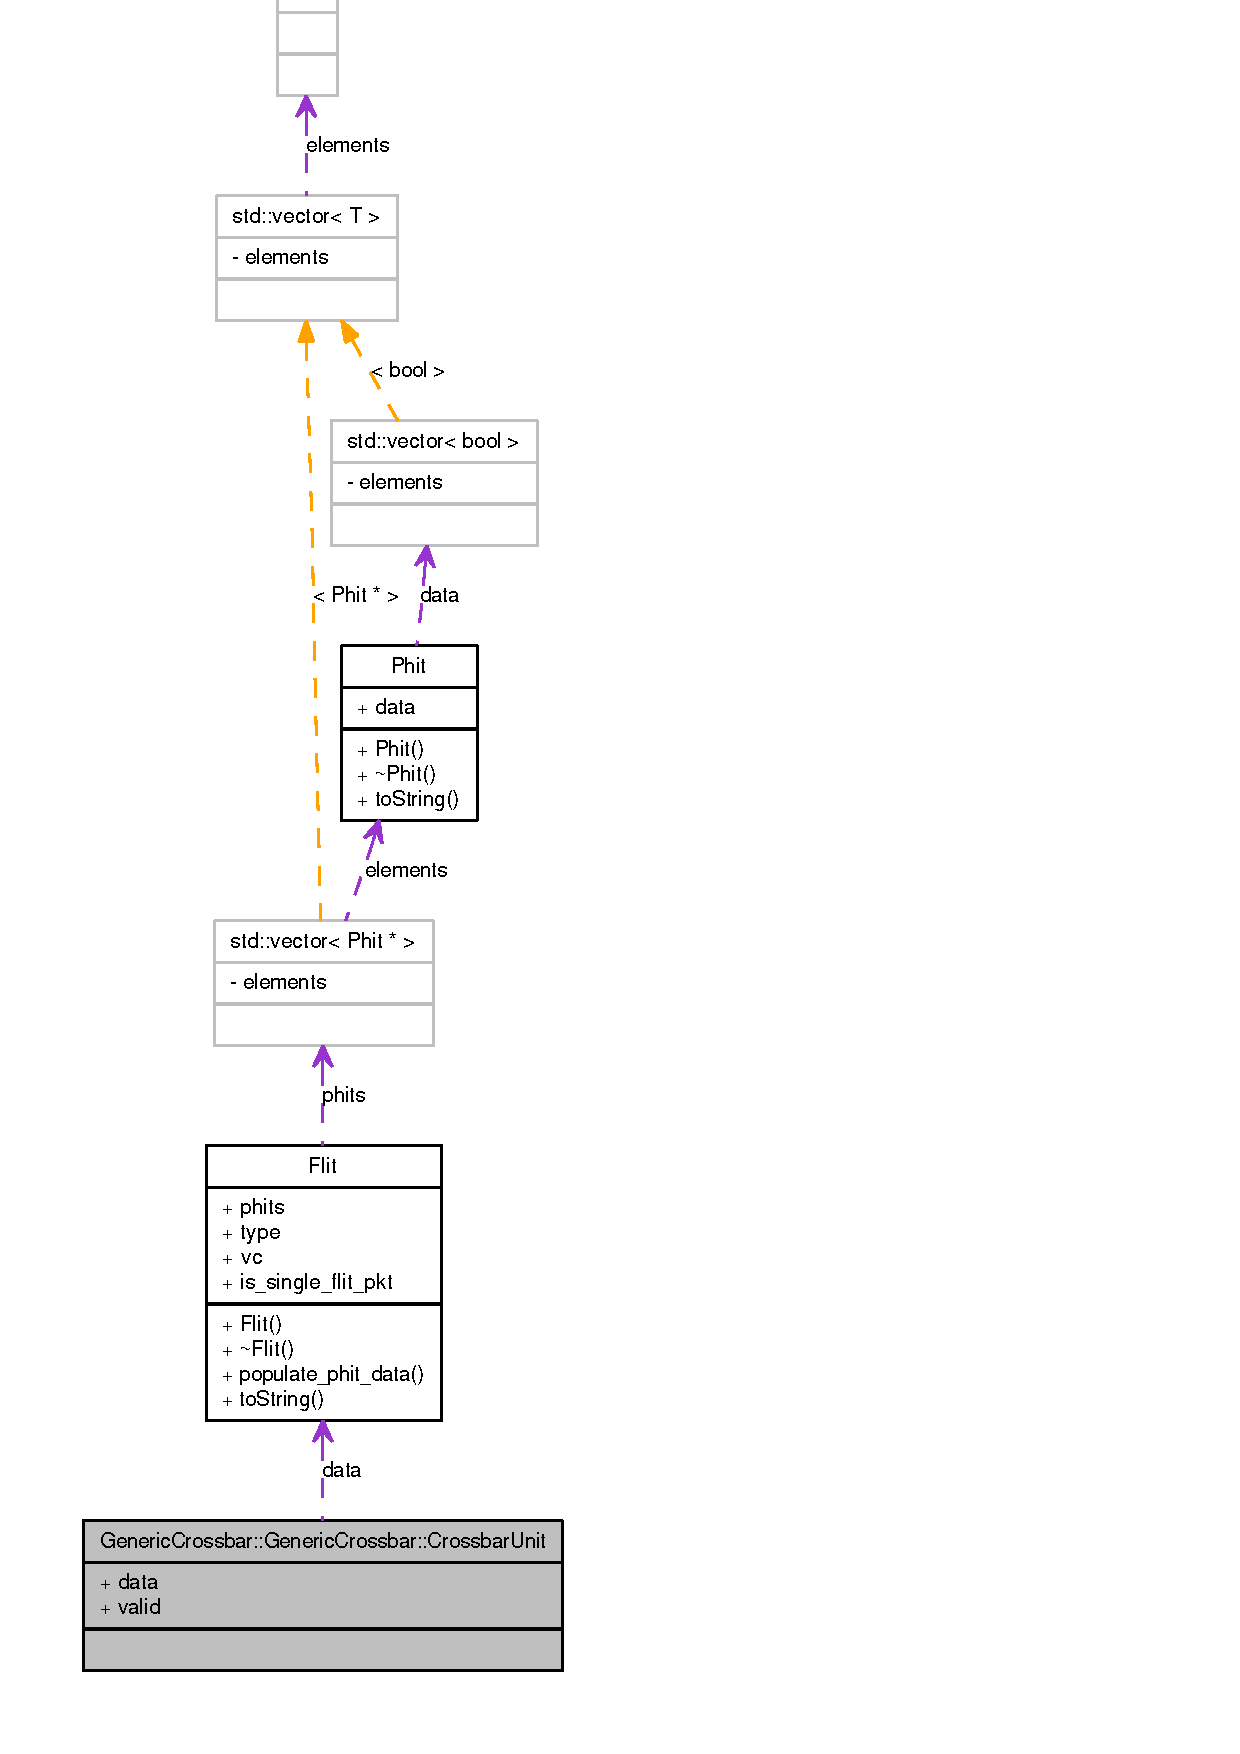
\includegraphics[height=400pt]{classGenericCrossbar_1_1CrossbarUnit__coll__graph}
\end{center}
\end{figure}
\subsection*{Public Attributes}
\begin{CompactItemize}
\item 
{\bf Flit} $\ast$ {\bf data}
\item 
bool {\bf valid}
\end{CompactItemize}


\subsection{Detailed Description}


Definition at line 65 of file genericCrossbar.h.

\subsection{Member Data Documentation}
\index{GenericCrossbar::CrossbarUnit@{GenericCrossbar::CrossbarUnit}!data@{data}}
\index{data@{data}!GenericCrossbar::CrossbarUnit@{GenericCrossbar::CrossbarUnit}}
\subsubsection[{data}]{\setlength{\rightskip}{0pt plus 5cm}{\bf Flit}$\ast$ {\bf GenericCrossbar::GenericCrossbar::CrossbarUnit::data}}\label{classGenericCrossbar_1_1CrossbarUnit_14558670755f9674e22592dd0d2ddd05}




Definition at line 68 of file genericCrossbar.h.\index{GenericCrossbar::CrossbarUnit@{GenericCrossbar::CrossbarUnit}!valid@{valid}}
\index{valid@{valid}!GenericCrossbar::CrossbarUnit@{GenericCrossbar::CrossbarUnit}}
\subsubsection[{valid}]{\setlength{\rightskip}{0pt plus 5cm}bool GenericCrossbar::GenericCrossbar::CrossbarUnit::valid}\label{classGenericCrossbar_1_1CrossbarUnit_46d03ff28869471ba9db56ca6acb3668}




Definition at line 69 of file genericCrossbar.h.

The documentation for this class was generated from the following file:\begin{CompactItemize}
\item 
{\bf genericCrossbar.h}\end{CompactItemize}
